\documentclass[a4paper, 12pt]{article}

\newcommand{\assignmentAuthor}{Bhaskar Goyal}
\newcommand{\course}{CSCI - 567}
\newcommand{\assignmentName}{HW 01}
\newcommand{\USCID}{6547367383}
\newcommand{\assignmentDate}{July 7, 2021}

\addtolength{\hoffset}{-2.25cm}
\addtolength{\textwidth}{4.5cm}
\addtolength{\voffset}{-2.5cm}
\addtolength{\textheight}{5cm}
\setlength{\parskip}{0pt}
\setlength{\parindent}{15pt}

\usepackage{amsthm}
\usepackage{amsmath}
\usepackage{amssymb}
\usepackage{bm}
\usepackage{tikz}
\usetikzlibrary{automata}
\usepackage{enumitem}
\usepackage{mathabx}
\usepackage{algorithmic}
\usepackage[colorlinks = true, linkcolor = black, citecolor = black, final]{hyperref}
\usepackage{tikz}
\usetikzlibrary{automata}

\usepackage{graphicx}
\usepackage{multicol}
\usepackage{ marvosym }
\usepackage{wasysym}
\usepackage{tikz}
\usetikzlibrary{patterns}
\usepackage{fancyhdr}
\usepackage{amssymb,latexsym,amsmath,amsthm}
\usepackage{amsfonts,rawfonts}
\usepackage{thmtools}
\usepackage{systeme}
\usepackage{mathtools}

\pagestyle{fancy}
\fancyhf{}
\rhead{\assignmentAuthor \; (USC ID - \USCID)}
\lhead{\course \; \assignmentName}
\rfoot{Page \thepage}
\lfoot{\assignmentDate}

\newcommand{\ds}{\displaystyle}

\setlength{\parindent}{0in}
\graphicspath{ {./images/} }

\declaretheoremstyle[
headfont=\color{blue}\normalfont\bfseries,
notefont=\bfseries, 
notebraces={}{},
% bodyfont=\color{red}\normalfont\itshape,
bodyfont=\normalfont,%\itshape,
%headformat=\NUMBER.~\NAME\NOTE
headformat=\NAME\NOTE
]{colorquestion}

\declaretheorem[
numbered=no,
style=colorquestion,
name=Question
]{question}

\title{\course \; \assignmentName}
\author{\textbf{\assignmentAuthor} \\ \Small{USC ID - \USCID}}
\date{\assignmentDate}

% ----------------------------

% The "stuff" above here is called the preamble of the document.  It sets the margins and loads special packages.  Probably the only reason you would need to edit something above here would be to add a package to do something very specific... but probably everything you need is loaded already

% -----------------------------

\begin{document}
\thispagestyle{plain}
\maketitle
\hrule
\bigskip

% -------------------------
% Question 1
% -------------------------

\begin{proof}[\color{red}{\textbf{Problem 1}: Decision Tree}]

\hfill

\begin{enumerate}[label={\color{blue}{\textbf{1.\arabic*})}}]
    \item 
        To calculate Test Error, we need to predict the test data points\\
        \textbf{Point 1:} $x_1 = 0.8, x_2 = 0.8, y = 0$ \\
        $y_{Predicted} = 0$ \\
        (Because, $x_1 > 0.5$ and $x_2 > 0.5$). \\
        $\therefore$ Point 1 is correctly classified. \\
        \textbf{Point 2:} $x_1 = 0.6, x_2 = 0.4, y = 1$ \\
        $y_{Predicted} = 1$ \\
        (Because, $x_1 > 0.5$ and $x_2 < 0.5$). \\
        $\therefore$ Point 2 is correctly classified. \\
        \textbf{Test Error}
        \begin{align*}
            \text{Test Error} &= \frac{\text{Misclassified Test Points}}{\text{Total Test Points}} \\
            &= \frac{0}{2} \\
            &= 0
        \end{align*} 
        Hence, the Test Error = 0
        
    \item 
        To calculate Test Error, we need to predict the test data points using the new Decision Tree from Figure 3 (in question). \\
        \textbf{Point 1:} $x_1 = 0.8, x_2 = 0.8, y = 0$ \\
        $y_{Predicted} = 1$ \\
        (Because, $x_1 > 0.5$). \\
        $\therefore$ Point 1 is misclassified. \\
        \textbf{Point 2:} $x_1 = 0.6, x_2 = 0.4, y = 1$ \\
        $y_{Predicted} = 1$ \\
        (Because, $x_1 > 0.5$. \\
        $\therefore$ Point 2 is correctly classified. \\
        \textbf{Test Error}
        \begin{align*}
            \text{Test Error} &= \frac{\text{Misclassified Test Points}}{\text{Total Test Points}} \\
            &= \frac{1}{2}
        \end{align*} 
        Hence, the Test Error = $1/2 = 0.5$
        
        
    \item 
        Yes, the decision tree in Figure 3 is a \textbf{linear} classifier in terms of $(x_1, x_2)$. This is because the condition on root node of decision tree is $x_1 > 0.5$ which is a linear equation in $x_1$.
        \smallskip
        
        No, we can't classify the given data in Table 1 and get zero classification error by drawing a depth-1 decision tree similar to Figure 3. This is because the data points are \textbf{non-linearly separable}. 
        
    
    \item
        Yes, because the data points are \textbf{non-linearly separable}, we can get zero classification error by putting any expression of variables like $f(x_1, x_2) \geq c$ or $f(x_1, x_2) \leq c$. \\
        This means, we can put a non-linear function equation which separate the data points into 2 distinct regions. \\
        Any elliptical or hyperbolic equation which separate the data points into 2 distinct regions will give zero error. \\
        Ex. Below is a ellipse equation which separate the data points. 
        \begin{align*}
            \frac{\left(\left(x-0.5\right)\cos\left(\frac{\pi}{4}\right)-\left(y-0.5\right)\sin\left(\frac{\pi}{4}\right)\right)^{2}}{1}+\frac{\left(\left(x-0.5\right)\sin\left(\frac{\pi}{4}\right)+\left(y-0.5\right)\cos\left(\frac{\pi}{4}\right)\right)^{2}}{\frac{1}{8}}<1
        \end{align*}
        \begin{center}
            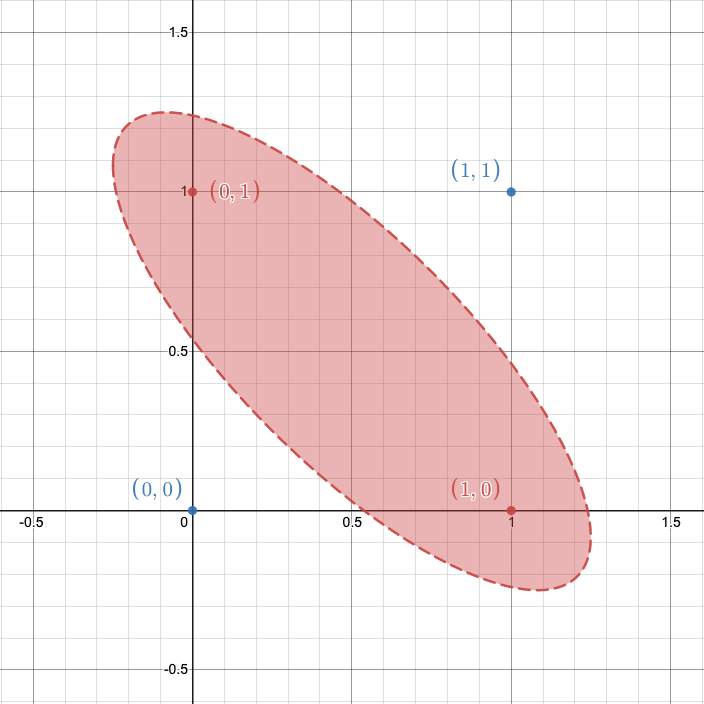
\includegraphics[scale=0.35]{Ellipse}
        \end{center}
\end{enumerate}
\end{proof}



% -------------------------
% Question 2
% -------------------------
\hrule
\bigskip
\pagebreak
\begin{proof}[\color{red}{\textbf{Problem 2}: kNN Classification}]

\hfill

\begin{enumerate}[label={\color{blue}{\textbf{2.\arabic*})}}]
    \item 
        \textbf{Given}: $P(y|x,x') = P(y|x)$ for any $x'$ \\
        \textbf{To prove}: $P(y,y'|x,x') = P(y|x)P(y'|x')$ 
        \smallskip
        
        \textbf{Proof:}
        \begin{align*}
            P(y,y'|x,x') &= P(y|y',x,x').P(y'|x',x) \tag*{(using Chain Rule)}\\
            &= P(y|y',x,x').P(y'|x') 
            \tag*{(using label independence)}\\
            &= P(y|y',x).P(y'|x') 
            \tag*{(using label independence)}\\
            &= P(y|x,y').P(y'|x') \\
            &= {P(y|x).P(y'|x')}  \tag*{(using label independence)} 
        \end{align*}
    Hence, proved.
        
    \item 
        \textbf{Given}: $n \to \infty,x_{\text{NN}} \text{ satisfies } ||x_{\text{NN}} - x_t|| \to 0$ \\
        \textbf{To prove}: $P(y^* \neq y|x_{\text{NN}},x_t) \to 2P(y^* = 0|x_t)P(y^* = 1|x_t)$ 
        \smallskip
        
        \textbf{Proof:}
        
        $P(y^* \neq y|x_{\text{NN}},x_t) $
        \begin{align*}
            &= P(y^*=0,y=1|x_{\text{NN}},x_t) + P(y^*=1,y=0|x_{\text{NN}},x_t)
            \\
            &= P(y^*=0|x_{\text{NN}},x_t).P(y=1|x_{\text{NN}},x_t) + P(y^*=1|x_{\text{NN}},x_t).P(y=0|x_{\text{NN}},x_t)
            \\
            \tag*{(using chain rule)}\\
            &= P(y^*=0|x_t).P(y=1|x_{\text{NN}}) + P(y^*=1|x_t).P(y=0|x_{\text{NN}})
            \\
            \tag*{(using label independence)}\\
            &= P(y^*=0|x_t).(1 - P(y=0|x_{\text{NN}})) + (1 - P(y^*=0|x_t)).P(y=0|x_{\text{NN}})
            \\
            \tag*{(summation of probabilities equals 1)}\\
            &\to P(y^*=0|x_t).(1 - P(y^*=0|x_t)) + (1 - P(y^*=0|x_t)).P(y^*=0|x_t)
            \\
            \tag*{(if $||x_{\text{NN}} - x_t|| \to 0$ then, $x_{\text{NN}} \to x_t$ and $y \to y^*$)}\\
            &\to 2P(y^*=0|x_t).(1 - P(y^*=0|x_t))
            \\
            &\to 2P(y^*=0|x_t).P(y^*=1|x_t) \tag*{(summation of probabilities equals 1)}
        \end{align*}
        Hence, proved.
        
    \item 
        \textbf{Given}: $P(y^* \neq y|x_{\text{NN}},x_t) \to 2P(y^*=0|x_t).P(y^*=1|x_t)$ \\
        \textbf{To Prove}: $P(y^* \neq y|x_{\text{NN}},x_t) \leq  \min\limits_y 2P(y|x_t)) $ 
        \smallskip
        
        \textbf{Proof:}
        
        In the given equation, $P(y^* \neq y|x_{\text{NN}},x_t) \to 2P(y^*=0|x_t).P(y^*=1|x_t)$
        
        We know that both the terms $P(y^*=0|x_t)$ and $P(y^*=1|x_t)$ are between [0,1]. And we also know that 
        
        if $0 \leq a, b \leq 1$ and $a \leq b$ then, $a.b < a$ and $a.b < b$ 
        
        Similarly, 
        \begin{align*}
            P(y^*=0|x_t).P(y^*=1|x_t) \leq \min\limits_y P(y|x_t) \tag*{(eq 1)}
        \end{align*}
        Using the above result,
        \begin{align*}
            P(y^* \neq y|x_{\text{NN}},x_t)  &\to 2P(y^*=0|x_t).P(y^*=1|x_t) \\
            &\leq  \min\limits_y 2P(y|x_t) \tag*{(using result in eq 1)}
        \end{align*}
        Hence, Proved.
        
    \item 
        For Bayes Optimal Classifier, $\min\limits_y P(y|x)$ denotes the Optimal risk/error. \\
        For NN Classifier, we know that $P(y^* \neq y|x_{\text{NN}},x_t)$ denotes the error/risk. 
        
        Let, \\
        $R(f_{\text{Bayes}})$ = optimal risk/error for bayes optimal classifier.\\
        $R(f_{\text{NN}})$ = risk/error for the NN classifier.
        
        Then, 
        \begin{align*}
            R(f_{\text{Bayes}}) &= \min\limits_y P(y|x) \\
        R(f_{\text{NN}}) &= P(y^* \neq y|x_{\text{NN}},x_t)
        \end{align*}
        
        
        
        Using the above results in $2.3$, we know that 
        \begin{align*}
            P(y^* \neq y|x_{\text{NN}},x_t) &\leq  \min\limits_y 2P(y|x_t)) \\
            R(f_{\text{NN}}) &\leq 2R(f_{\text{Bayes}})
        \end{align*}
        
        $\therefore$ $\min\limits_y P(y|x)$ denotes the optimal risk/error for the bayes optimal classifier. And the risk/error involved in NN classification is atmost twice involved in the Bayes optimal classifier. 
    
\end{enumerate}
\end{proof}


% -------------------------
% Question 3
% -------------------------
\hrule
\bigskip

\begin{proof}[\color{red}{\textbf{Problem 3}: Boosting (Adaboosting)}]

\hfill

\begin{enumerate}[label={\color{blue}{\textbf{3.\arabic*})}}]
    \item 
        Two rounds of boosting \\
        
        \underline{\textbf{Round 1 Calculations}:}
        
        
        \textit{\textbf{Initial weights}} will be all equally distributed. Hence, all 6 training sample's weights will get 1/6 value.
        \begin{align*}
            \text{weight}_{A, B, C, D E, F}  &= 1/6
        \end{align*}
        
        \textit{\textbf{Error rate}} will the weighted average of miss classified label weights. There values will be as follows:
        \begin{align*}
            \text{Error of h1} &= \frac{1}{6}.3 = \frac{3}{6}\\
            \text{Error of h2} &= \frac{1}{6}.1 = \frac{1}{6}\\
            \text{Error of h3} &= \frac{1}{6}.2 = \frac{2}{6}\\
            \text{Error of h4} &= \frac{1}{6}.3 = \frac{3}{6}\\
            \text{Error of h5} &= \frac{1}{6}.3 = \frac{3}{6}\\
        \end{align*}
        
        
        \textit{\textbf{Weak Classifier:}} The least error rate is of the h2 classifier in round 1. Hence, it's respective values will be 
        
        \begin{align*}
            \text{Weak Classifier (h)} &= \text{h2}\\
            \text{Classifier Error ($\epsilon $)} &=  \frac{1}{6}  \\
            \text{Voting power} (\alpha)  &= \frac{1}{2}.\ln{\frac{1 - \epsilon}{\epsilon}} \\  
                    &= \frac{1}{2}.\ln{\frac{1 - (1/6)}{(1/6)}} \\ 
                    &= \frac{1}{2}.\ln{5}  
        \end{align*}
        
        \underline{\textbf{Round 2 Calculations}:}
        
        \textit{\textbf{Weights:}}
        
        The formula for calculating weights for the next round is given by
        \begin{align*}
        \text{weight}_{t+1}(n) = \text{weight}_t(n).e^{-\alpha_ty_nh_t(x_n)} = \begin{cases}
   \text{weight}_t(n).e^{-\alpha_t}& \text{if }h_t(x_n)=y_n\\    
   \text{weight}_t(n).e^{\alpha_t}& \text{otherwise}
\end{cases}
        \end{align*}
        
        Using it for calculating the new weights of round 2, 
        \begin{align*}
            \text{weight}_{A, B, C, E, F \text{ (Not Normalized)}}  &= w_{\text{Round 1}}.e^{-{\frac{1}{2}.\ln\frac{1-\epsilon}{\epsilon}}} \\
                    &= \frac{1}{6}.e^{-{\frac{1}{2}.\ln\frac{1-(1/6)}{(1/6)}}} \\  
                    &= \frac{1}{6}.e^{-{\frac{1}{2}.\ln 5}} \\  
                    &= \frac{1}{6\sqrt{5}}
        \end{align*}
        \begin{align*}
            \text{weight}_{D  \text{ (Not Normalized)}}  &= w_{\text{Round 1}}.e^{{\frac{1}{2}.\ln\frac{1-\epsilon}{\epsilon}}} \\
                    &= \frac{1}{6}.e^{{\frac{1}{2}.\ln\frac{1-(1/6)}{(1/6)}}} \\  
                    &= \frac{1}{6}.e^{{\frac{1}{2}.\ln 5}} \\  
                    &= \frac{\sqrt{5}}{6}
        \end{align*}
        \begin{align*}
            \text{Total Weight =}& \text{ weight}_{A} + \text{ weight}_{B} + \text{ weight}_{C} + \text{ weight}_{D} + \text{ weight}_{E} + \text{ weight}_{F}\\
            =& 5(\frac{1}{6\sqrt{5}}) + \frac{\sqrt{5}}{6}\\
            =& \frac{2\sqrt{5}}{6}
        \end{align*}
        \begin{align*}
            \text{weight}_{A, B, C, E, F \text{ (Normalized)}}  &= \frac{w_{\text{A, B, C, E, F Not Normalized}}}{\text{Total Weight}} \\
                    &= \frac{1}{6\sqrt{5}} / \frac{2\sqrt{5}}{6}\\
                    &= \frac{1}{10}
        \end{align*}
        \begin{align*}
            \text{weight}_{D \text{ (Normalized)}}  &= \frac{w_{\text{D, Not Normalized}}}{\text{Total Weight}} \\
                    &= \frac{\sqrt{5}}{6} / \frac{2\sqrt{5}}{6}\\
                    &= \frac{1}{2}
        \end{align*}
        
        \textit{\textbf{Error rate}} will the weighted average of miss classified label weights. There values will be as follows:
        \begin{align*}
            \text{Error of h1} &= \frac{1}{10}.2 + \frac{1}{2}.1 = \frac{7}{10}\\
            \text{Error of h2} &= \frac{1}{2}.1 = \frac{1}{2} = \frac{5}{10}\\
            \text{Error of h3} &= \frac{1}{10}.2 = \frac{2}{10}\\
            \text{Error of h4} &= \frac{1}{10}.3 = \frac{3}{10}\\
            \text{Error of h5} &= \frac{1}{10}.2 + \frac{1}{2}.1 = \frac{1}{2} = \frac{7}{10}
        \end{align*}
        
        \textit{\textbf{Weak Classifier:}} The least error rate is of the h3 classifier in round 2. Hence, it's respective values will be 
        
        \begin{align*}
            \text{Weak Classifier (h)} &= \text{h3}\\
            \text{Classifier Error ($\epsilon $)} &=  \frac{2}{10} = \frac{2}{10}  \\
            \text{Voting power} (\alpha)  &= \frac{1}{2}.\ln{\frac{1 - \epsilon}{\epsilon}} \\  
                    &= \frac{1}{2}.\ln{\frac{1 - (2/10)}{(2/10)}} \\ 
                    &= \frac{1}{2}.\ln{4}  
        \end{align*}
        
        \textit{\textbf{Table}}
        
        \begin{center}
            \begin{tabular}{|l|c|c|}
            \hline
                                & Round 1 & Round 2 \\ \hline
            $\text{weight}_A$              &    $1/6$     &     
            $1/10$              \\ \hline
            $\text{weight}_B$              &    $1/6$     &    $1/10$       \\\hline
            $\text{weight}_C$              &    $1/6$     &    $1/10$       \\\hline
            $\text{weight}_D$              &    $1/6$     &    $1/2$      \\\hline
            $\text{weight}_E$              &    $1/6$     &    $1/10$       \\\hline
            $\text{weight}_F$              &    $1/6$     &    $1/10$       \\\hline\hline
            Error rate of h1    &    $3/6$     &  7/10       \\\hline
            Error rate of h2    &    $1/6$     &  5/10       \\\hline
            Error rate of h3    &    $2/6$     &  2/10       \\\hline
            Error rate of h4    &    $3/6$     &  3/10       \\\hline
            Error rate of h5    &    $3/6$     &  7/10       \\\hline\hline
            weak classifier (h) &   h2  &     h3    \\\hline
            classifier error ($\epsilon$) &    $1/6$     &   $2/10$      \\\hline
            voting power ($\alpha$)        &    
                $\frac{1}{2}.\ln{5}$ 
            &     $\frac{1}{2}.\ln{4}$      \\ \hline
            \end{tabular}
        \end{center}
        
    \item 
        For classification, the training point will be the weighted average of the voting power of the weak classifiers of each round. i.e. h2 and h3
        \begin{align*}
                H(x) &= \alpha_1h2 + \alpha_2h3 = \frac{1}{2}\ln5(h2) + \frac{1}{2}\ln4(h3)\\
                \text{Training Point B: } &= \frac{1}{2}\ln5 - \frac{1}{2}\ln4 \;> 0 \;\;\; \text{(Correctly Classified)}\\
                \text{Training Point D: } &= -\frac{1}{2}\ln5 + \frac{1}{2}\ln4 \;< 0 \;\;\; \text{(Misclassified)}\\
                \text{Training Point F: } &= \frac{1}{2}\ln5 + \frac{1}{2}\ln4 \;> 0 \;\;\; \text{(Correctly Classified)}
        \end{align*}
        \begin{center}
            \begin{tabular}{|l|l|l|l|}
            \hline
            Training Point & \multicolumn{3}{l|}{Classification by ensemble classifier}                                      \\ \hline
            B              & {\color[HTML]{000000} \textbf{Correctly classified}}                        & Misclassified & Can't tell \\ \hline
            D              & Correctly classified & {\color[HTML]{000000} \textbf{Misclassified}}                        & Can't tell \\ \hline
            F              & {\color[HTML]{000000} \textbf{Correctly classified}}                        & Misclassified & Can't tell \\ \hline
            \end{tabular}
        \end{center}
        
        
    \item 
        \bm{$E$} training point will have the smallest weight at the end of the 2021st round. \\
        This is because $E$ was never misclassified by any classifier in any round. Hence, it's importance (or weight) will be the least among all the training data points.
    
\end{enumerate}
\end{proof}
\hrule
\bigskip

\end{document}
